In this section, we focus on 2 points; Our meat-model being of considerable size, explaining it as separate core packages, gives a better understanding and overview of the complete model. Secondly, we explain the key concepts behind the definition of policies.
 
By using Eclipse~\cite{eclipse}, EMF~\cite{emf} and Xtext~\cite{xtext} we built a domain specific language that is rich enough to express the policies discovered in the analysis. We developed a grammar that is based on our programming experience, and believed to have a consistent forthcoming syntax and conceptual constructs. Finally, we used our Policy Engine DSL editor to specify buildings and write the policies. The full DSL implementation based on two of the interviews, one for Br\"{u}el \& Kj\ae r (see Figure \nameref{app:bogk}) and one for K\o benhavns Tekniske Skole (see Figure \nameref{app:kts}). Please note that they are fully working implementations running in Eclipse.

\subsection{Meta-Models}

The following core packages, differentiated in separate Ecore Diagrams (can be viewed in full in \nameref{app:a-metamodel}); 9 sensors classes and 6 actuators classes (see Figure \ref{fig:ecore-sensors-actuators}), 14 expression language classes (see Figure \ref{fig:ecore-expression-language}), 4 building definition classes (see Figure \ref{fig:ecore-building-definition}) and 10 policy definition classes (see Figure \ref{fig:ecore-policy-definition}).

\subsubsection{Sensors and Actuators}
in our metamodel and used in our DSL are from the combined analysis of the interview mentioned in the section above. Sensor and Actuator class inherit from NamedElement, giving declared elements a name than can be later referenced in the expression language.
\begin{figure}[h]
	\centering
    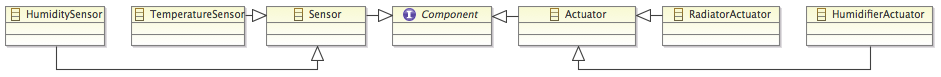
\includegraphics[scale=.45]{ecore-sensors-actuators.png} 
	\caption{A fragment of the \textit{sensor} and \textit{actuator} metamodel hierarchy. If new types are needed, they should be defined in the metamodel.}
	\label{fig:ecore-sensors-actuators}
\end{figure}

\subsubsection{Building definition}
In order to specify the building(s) with all their floors and rooms, the core classes has been included in Figure \ref{fig:ecore-building-definition}. They all inherit from NamedElement, making it possible to give them a name than can be used for later referencing.
\begin{figure}[h]
  \centering 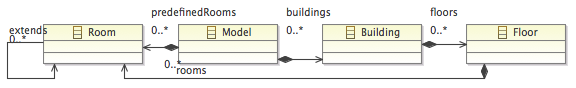
\includegraphics[scale=.5]{ecore-building-definition.png}  
	\caption{The metamodel related to the \textit{building definition}. The inherited class NamedElement has been omitted.}
	\label{fig:ecore-building-definition}
\end{figure}

\subsubsection{Expression language}
After the analysis of the interviews we concluded that the needed expression language did not need to be very advanced. We needed boolean variables (\textit{states}) and if-statements with two different types of conditions; the normal if-statement, which operates on sensor types and state instances. The other one operates on a timer (see Figure \ref{fig:dsl-conditionalexpression}). In the body of the if-statement, we can use expression to reset timers, and set actuators using instances in specific rooms as shown in the DSL example \ref{fig:dsl-policy-definition}

\begin{figure}[h]
  \centering
    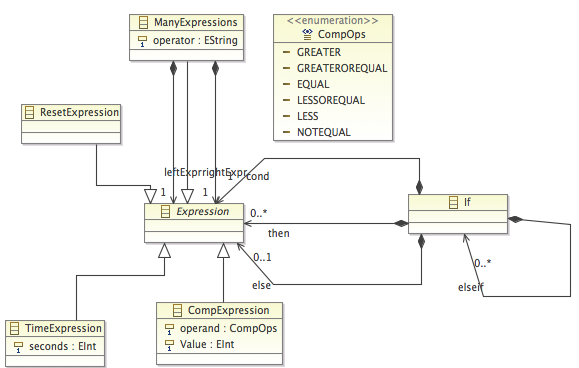
\includegraphics[scale=.5]{ecore-expression-language.png} 
	\caption{The metamodel related to the \textit{expression language}. The inherited class NamedElement has been omitted.}
	\label{fig:ecore-expression-language}
\end{figure}

\subsubsection{Policy definition}
In the policy definition metamodel below, to define a policy, we make use of actuator and sensor types, and use room instances. The implementation of the policy is enhanced by the use of statements; if, state and timer. the if-statement uses the expression language to define behaviour. These policy can also be run following a defined schedule as shown in the dsl example of room-type in figure \ref{fig:room-types} 
\begin{figure}[h]
  \centering
    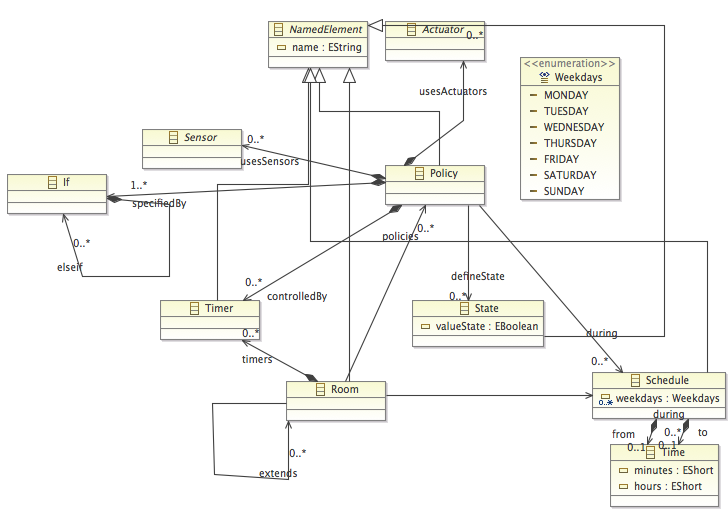
\includegraphics[scale=.5]{ecore-policy-definition.png}	
	\caption{The metamodel related to the \textit{policy definition}.}
	\label{fig:ecore-policy-definition}
\end{figure}

There are several extra classes, consisting of subsystems that can be implemented in Section \ref{sec:futureWork}.

\subsection{Key Concepts}

During the analysis of the interviews, different meta-constructs were defined. It was evident that the three key concepts below were needed in order to tailor the policies for the interviewees using the DSL;

\subsubsection{Time}\label{subsec:time}
Time has to be an integral part of the DSL, and not just related with the internal policy logic. Several interviewees mention concepts like weekdays, weekends, normal working hours, holidays, night, day, morning etc., which clearly shows that Time is necessary. We have extrapolated the need for Time in two different cases;
\begin{enumerate}
	\item Time conditional expression\label{subsubsec:conditionalexpression}
A \textit{time conditional expression} is an expression used for determining the flow of a behavior. It is an `if' statement that can react based on a built-in timer function. 

\begin{figure}[h]
  \centering
    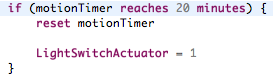
\includegraphics[scale=.5]{dsl-conditional-time-expression.png}
	\caption{An example of a \textit{time conditional expression} that evaluates to true if more than 20 minutes have passed.}
	\label{fig:dsl-conditionalexpression}
\end{figure}

\item Schedules\label{subsubsec:schedules}
\textit{Schedules} are predefined types representing a timespan, which can later be attached to a specific behavior where action or no-action takes place. Note that by defining several The \textit{schedules}, it is possible both to make schedules than can overlap in time, but also policies that takes over when other policies reach their end. 

\begin{figure}
  \centering
  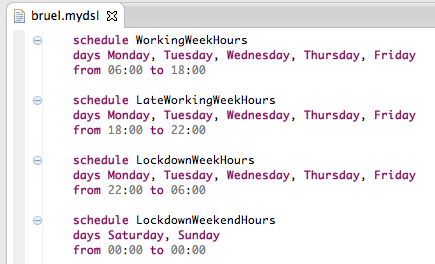
\includegraphics[scale=.5]{dsl-schedules.png}
  \caption{An example of a \textit{schedule} defined for a interviewee.}
  \label{fig:dsl-schedules}
\end{figure}
\end{enumerate}
\subsubsection{Building specification}\label{subsec:buildingspecification}
Rooms and room types are part of the complete building specification, with terminology rooted in concepts revolving around buildings, ie. rooms, room types, floors, different sensors and actuators. \\

To avoid confusing the DSL user with an overwhelming amount of declarations of rooms, sensors and actuators - we have designed \textit{room types} that declare static use of sensors and actuators. Independent rooms that stick out from the crown can still be defined on an instance level.

\begin{figure}
  \centering
    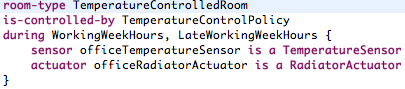
\includegraphics[scale=.5]{dsl-room-types.png}
	\caption{An example of \textit{room types} defined for a interviewee.}
	\label{fig:room-types}
\end{figure}

Building specification as in the example above, helps us map out the actual buildings as they are in our DSL. With this we are able to accurately define exact locations for sensors and actuators as well as implement policies for rooms in specific locations. 

\begin{figure}
  \centering
  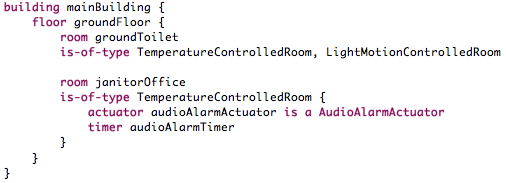
\includegraphics[scale=.5]{dsl-building-definition.png}  
  \caption{An example of \textit{building specification} defined for a interviewee. Note that the janitorOffice inherits from a TemperatureControlled room (which uses a \textit{TemperatureSensor} and a \textit{RadiatorActuator}) but also declares a \textit{AudioAlarmActuator} and a \textit{Timer} instance.}
  \label{fig:dsl-building-definition}
\end{figure}

\subsubsection{Policy}\label{subsec:policies}
Policies define the actual behavior, ie. adjustment of actuators, based on sensor input. In the dsl example below, when the humiditySensor value drops under 50, the humidityAlarm state is set to true and every 15 seconds of the timer, the audioAlarmActuator sets off the alarm in the janitorOffice.

\begin{figure}[h]
  \centering
    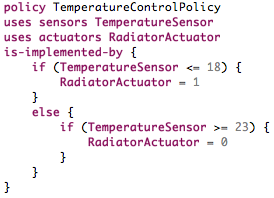
\includegraphics[scale=.5]{dsl-policy-definition.png} 
	\caption{An example of \textit{policy} using a single sensor type, a single actuator type and a room instance.}
	\label{fig:dsl-policy-definition}
\end{figure}